%% LyX 2.1.4 created this file.  For more info, see http://www.lyx.org/.
%% Do not edit unless you really know what you are doing.
\documentclass[11pt,french]{article}
\usepackage[T1]{fontenc}
\usepackage[utf8]{inputenc}
\usepackage{geometry}
\geometry{verbose,tmargin=3cm,bmargin=3cm,lmargin=3cm,rmargin=3cm}
\usepackage{babel}
\makeatletter
\addto\extrasfrench{%
   \providecommand{\og}{\leavevmode\flqq~}%
   \providecommand{\fg}{\ifdim\lastskip>\z@\unskip\fi~\frqq}%
}

\makeatother
\usepackage{float}
\usepackage{graphicx}
\usepackage{setspace}
\doublespacing
\usepackage[unicode=true,
 bookmarks=false,
 breaklinks=false,pdfborder={0 0 1},backref=section,colorlinks=false]
 {hyperref}
\hypersetup{
 colorlinks,linkcolor=black,urlcolor=black}
\usepackage{breakurl}

\makeatletter
%%%%%%%%%%%%%%%%%%%%%%%%%%%%%% User specified LaTeX commands.
\usepackage{babel}


%\usepackage[french]{babel}



\usepackage{svg}

\makeatother

\begin{document}
\begin{titlepage}\par \global\long\def\HRule{\rule{\linewidth}{1mm}}
 % Defines a new command for the horizontal lines, change thickness here
\center % Center everything on the page
 %----------------------------------------------------------------------------------------
%	HEADING SECTIONS
%----------------------------------------------------------------------------------------
\textsc{\LARGE Génie Mathématique 4ème année}\\[1.5cm] % Name of your university/college
\textsc{\Large Projet Semestriel}\\[0.5cm] % Major heading such as course name
\textsc{\large C++}\\[0.5cm] % Minor heading such as course title
%----------------------------------------------------------------------------------------
%	TITLE SECTION
%----------------------------------------------------------------------------------------
\HRule \\[0.5cm] { \huge \bfseries Le Tarot }\\[0.4cm] % Title of your document
\HRule \\[1.5cm]\par %----------------------------------------------------------------------------------------
%	AUTHOR SECTION
%----------------------------------------------------------------------------------------
\begin{minipage}[c]{0.4\textwidth}%
\begin{flushleft}
\emph{\large{}{}Auteurs:}{\large{}{}}\\
 {\large{}{} }\textsc{\large{}{}Ahmed Farouk BELGHAZI }{\large{}}\\
{\large{} }\textsc{\large{}{}Gabriel DUFLO}{\large{}}\\
{\large{} }\textsc{\large{}{}Adrien LATIL}{\large{}}\\
{\large{} }\textsc{\large{}{}Nicolas LEGOUY}{\large{}}\\
{\large{} }\textsc{\large{}{}Nicolas MONANGE}{\large{}{} % Your name
} 
\par\end{flushleft}

%
\end{minipage}~ %
\begin{minipage}[c]{0.4\textwidth}%
\begin{flushright}
\emph{\large{}{}Superviseurs:}{\large{}{} }\\
 {\large{}{} }\textsc{\large{}{}Cécilia ZANNI-MERK}{\large{}}\\
{\large{} }\textsc{\large{}{}Zina EL GUEDRIA SGAIER}{\large{}{}
% Supervisor's Name
} 
\par\end{flushright}

%
\end{minipage}\\[2cm]\par %----------------------------------------------------------------------------------------
%	DATE SECTION
%----------------------------------------------------------------------------------------
{\today}\\[2cm]\par %----------------------------------------------------------------------------------------
%	LOGO SECTION
%----------------------------------------------------------------------------------------

\includegraphics[width=0.8\textwidth]{insa_rouen}\par %----------------------------------------------------------------------------------------
\vfill{}
 \end{titlepage}

\tableofcontents{}\newpage{}


\part{Spécification}


\section{Règles du jeu}

Le tarot est un jeu basé sur le pari, de sorte que l'objectif est
de réussir à obtenir un certain nombre de points, annoncé à l'avance,
par un joueur dit \textbf{preneur}. Il peut en cela être aidé par
des cartes spéciales, les \textbf{bouts}. Suivant le nombre de joueurs
(3, 4 ou 5), le preneur peut jouer seul ou avec un partenaire. Cette
équipe est appelée le \textbf{Camp Déclarant}, tandis que les autres
joueurs représentent la \textbf{Défense}.


\subsection*{Les cartes}

Le tarot est un jeu composé de 78 cartes : 
\begin{itemize}
\item[$\bullet$] 14 cartes par couleur 
\item[$\bullet$] 21 atouts 
\item[$\bullet$] l'Excuse 
\end{itemize}
Dans chaque couleur, l'ordre des cartes est le suivant : 1-2-...-10-valet-cavalier-dame-roi.
Les atouts sont numérotés de 1 à 21 et sont prioritaires sur les cartes
de couleurs. Les bouts (au nombre de 3) sont des cartes spéciales
valant plus de points lors du comptage : 
\begin{itemize}
\item[$\bullet$] le 1 d'atout (aussi appelé le Petit) 
\item[$\bullet$] le 21 d'atout 
\item[$\bullet$] l'Excuse 
\end{itemize}
L'objectif de points dépend du nombre de bouts remportés à la fin
de la partie par le Camp Déclarant : 
\begin{itemize}
\item[$\bullet$] sans bout, l'objectif est de 56 points 
\item[$\bullet$] avec 1 bout, l'objectif est de 51 points 
\item[$\bullet$] avec 2 bouts, l'objectif est de 41 points 
\item[$\bullet$] avec 3 bouts, l'objectif est de 36 points 
\end{itemize}
Chaque carte vaut ainsi un certain nombre de points : 
\begin{itemize}
\item[$\bullet$] un bout : 4.5 points 
\item[$\bullet$] un roi : 4.5 points 
\item[$\bullet$] une dame : 3.5 points 
\item[$\bullet$] un cavalier : 2.5 points 
\item[$\bullet$] un valet : 1.5 point 
\item[$\bullet$] une petite carte (le reste) : 0.5 point 
\end{itemize}

\subsection*{Initialisation de la partie}

Un joueur désigné comme le donneur distribue les cartes 3 par 3 et
constitue le \textbf{chien} pendant la distribution. Ce dernier est
constitué de 6 cartes dans le cas d'une partie à 3 ou 4 joueurs et
de 3 cartes avec 5 joueurs. L'ensemble des cartes est alors distribué.
Chaque joueur regarde ses cartes tandis que le chien reste inconnu
(il est dévoilé à la fin des annonces). À la fin de la distribution,
chaque joueur, en commençant par celui à la gauche du donneur, va
faire une annonce en fonction de son jeu. Celle-ci va impacter le
score obtenu en fin de partie : 
\begin{itemize}
\item[$\bullet$] une \textbf{petite} : pas de bonus supplémentaire 
\item[$\bullet$] une \textbf{garde} : le résultat du pari est multiplié par 2 
\item[$\bullet$] une \textbf{garde sans le chien} (le chien n'est pas dévoilé et ses
cartes seront pour le Camp Déclarant) : le résultat du pari est multiplié
par 4 
\item[$\bullet$] une \textbf{garde contre le chien} (le chien n'est pas dévoilé et
ses cartes seront pour la Défense) : le résultat du pari est multiplié
par 6 
\end{itemize}
Le preneur est celui qui fait la plus grosse annonce. Si aucun joueur
ne fait d'annonce, les cartes sont redistribuées. Le multiplicateur
est donné en cas de victoire mais également en cas de défaite, d'où
le risque de prendre. Le preneur dévoile alors le chien (sauf dans
le cas d'une garde sans ou d'une garde contre) et place ses cartes
dans son jeu. Il crée ensuite un nouveau chien (sans que les autres
ne le voient) dont les cartes seront pour la Camp Déclarant (le preneur
n'a pas le droit de placer de bouts dans le chien et il peut placer
des rois seulement s'il le dit aux autres). Dans le cas d'une partie
à 5, le preneur choisit un roi, dont le propriétaire deviendra alors
son partenaire.


\subsection*{Déroulement}

C'est toujours le joueur situé à gauche du donneur qui commence la
partie. Il joue une couleur et les autres joueurs ont l'obligation
de fournir la couleur demandée si, bien entendu, ils en possèdent
les cartes. S'ils n'en possèdent pas, ils peuvent couper à l'atout.
Si un atout est joué en début de tour, les autres joueurs doivent
également jouer un atout mais toujours de valeur supérieur (s'ils
en possèdent les cartes).

Le gagnant du pli est celui qui a posé la carte de la couleur ouverte
ayant la plus grosse valeur si aucun atout n'a été posé, sinon c'est
celui qui a posé le plus gros atout. Dans le cas où l'Excuse est jouée,
le joueur ne fait pas le pli mais il conserve sa carte (sauf si elle
est jouée au dernier tour : dans ce cas, l'Excuse est remportée par
celui qui remporte le pli). Il donne en échange une petite carte depuis
sa pile. Celui qui gagne le pli ouvre le tour suivant.


\subsection*{Décompte des points}

Après que toutes les cartes ont été jouées, le Camp Déclarant compte
ses points et voit s'il a atteint son objectif. La somme de tous les
points faisant toujours 91, la Défense peut également compter ses
points pour en déduire le score du Camp Déclarant. Pour connaître
le résultat, il faut prendre la différence entre l'objectif et le
score. À ce nombre s'ajoutent alors 25 points. Enfin, il faut multiplier
le nombre obtenu par le coefficient correspondant à l'annonce. Ce
résultat est alors ajouté ou retranché aux joueurs de la Défense suivant
la réussite de l'objectif. Les joueurs du Camp Déclarant se partagent
ensuite les points de sorte que la somme des points de tous les joueurs
soit nulle. \\


\noindent \underline{Exemple :}

Si le Camp Déclarant fait 46 points avec 2 bouts, et a annoncé une
garde. Il dépasse son objectif de 5 points, auxquels s'ajoutent 25
points, ce qui donne 30 points. Étant donné que le preneur a annoncé
une garde, le résultat total est donc de $30*2=60$ points. Si le
preneur a joué seul, il empoche la totalité des points, sinon (dans
une partie à 5 joueurs, 2 pour le Camp Déclarant et 3 pour la Défense)
il prend 2/3 des points restants tandis que le partenaire en garde
1/3. Dans cas, dans une partie à 5, le preneur gagne alors 120 points
et le partenaire 60 points. La somme des points est bien nulle : $120+60+(-60)+(-60)+(-60)$.

Dans les mêmes conditions, si le Camp Déclarant avait marqué 36 points
(5 points en dessous de l'objectif), le preneur aurait marqué -120
points, son partenaire -60 points, et les joueurs de la Défense auraient
tous marqué 60 points.


\section{Diagramme des cas d'utilisations}

\begin{figure}[H]
\center 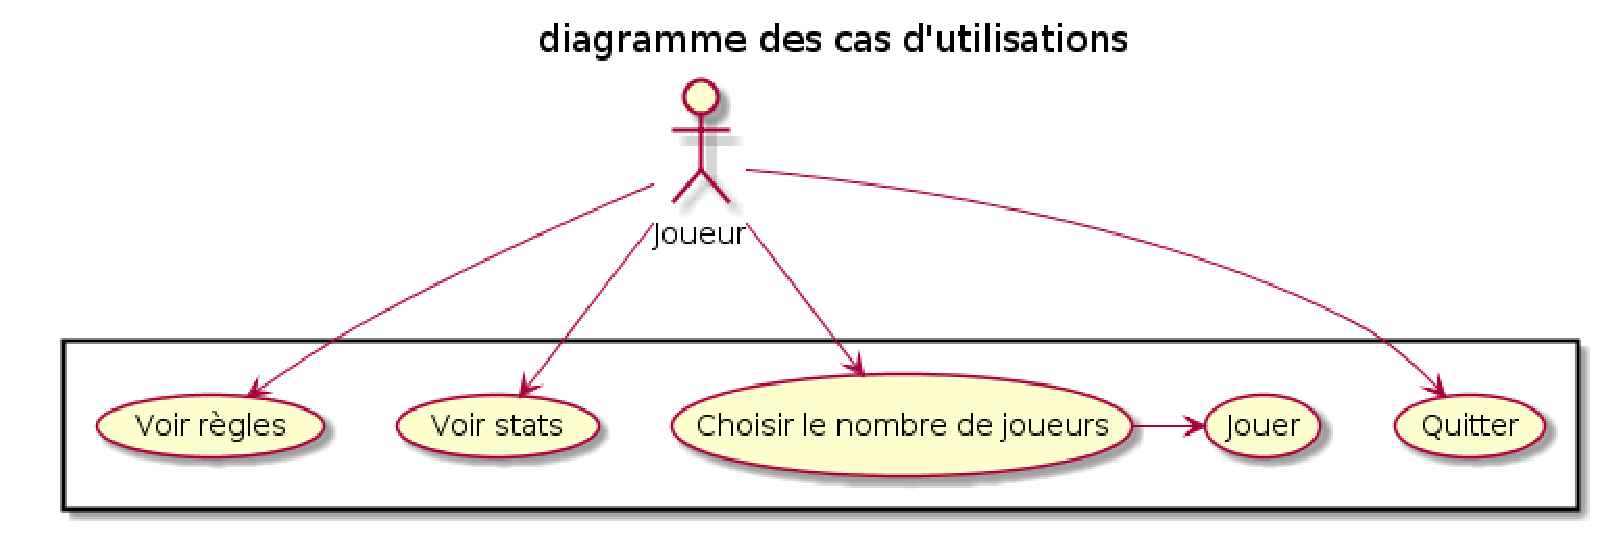
\includegraphics[scale=0.5]{cas_utilisations} \caption{Diagramme des cas d'utilisations}
\end{figure}



\section{Modèle du domaine}

\begin{figure}[H]
\center 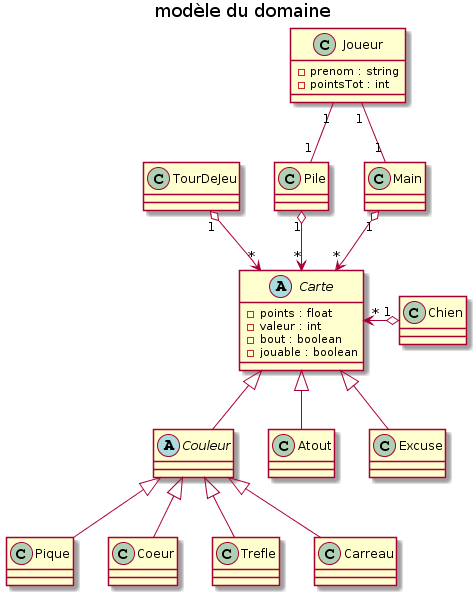
\includegraphics[scale=0.45]{modele_domaine} \caption{Modèle du domaine}
\end{figure}


Notre domaine se décompose en plusieurs classes : 
\begin{itemize}
\item[$\bullet$] la classe Joueur, qui contient le nom du joueur ainsi que son nombre
total de points, qui évolue à la fin de chaque partie en fonction
des résultats de la partie. Pendant la partie, le joueur possède une
Pile et une Main. 
\item[$\bullet$] la classe Pile représente les cartes remportées par le joueur au
sein d'une partie, stockées dans une liste de Carte. A la fin de chaque
tour de jeu, une fois que chaque joueur a déposé sa carte, le joueur
possédant la carte la plus forte remporte le pli, et ainsi les cartes
du tour de jeu sont placées dans la liste de sa pile. A la fin de
la partie, c'est en comptabilisant le nombre de points contenu dans
la pile de chaque joueur qu'on peut déterminer les résultats de la
partie. 
\item[$\bullet$] la classe Main représente les cartes que le joueur à en main et qu'il
peut donc potentiellement jouer au tour de jeu suivant. Ces cartes
sont contenues dans une liste de Carte, qui perd un élément à chaque
tour de jeu, et qui est vide à la fin de la partie. 
\item[$\bullet$] la classe abstraite Carte représente l'ensemble des cartes du jeu
; elle possède en paramètre le nombre de points que vaut la carte
(pour la comptabilisation des points à la fin de la partie), un booléen
indiquant si la carte considérée est un bout (3 cartes auront ce booléen
a « true », il sera « false » pour toutes les autres), un entier valeur
qui correspond à la valeur de la carte ( par exemple 5 pour le 5 de
carreau, 14 pour une dame, 7 pour l'atout 7... Et 0 par défaut pour
l'excuse), et un booléen jouable qui indique a chaque tour de jeu
quelles cartes peuvent être jouées, en accord avec les règles du jeu.
Nous avons divisé les cartes en 3 classe différentes, qui héritent
chacune de cette classe abstraite. 
\item[$\bullet$] la classe Atout, représente une carte atout. Il y a 21 cartes de
classe Atout, avec le 1 et le 21 qui auront le booléen « bout » à
« true ». 
\item[$\bullet$] la classe Excuse, qui représente la carte excuse et qui aura donc
le booléen « bout » à « true ». 
\item[$\bullet$] la classe abstraite Couleur, représente l'ensemble des cartes de
couleur, c'est à dire toutes les cartes de Trèfle, Carreau, Pique
et Cœur. Chacune de ces classes hérite de la classe abstraite Couleur
et représente les 14 cartes de cette couleur. 
\item[$\bullet$] la classe TourDeJeu représente les cartes jouées par les joueurs
au tour de jeu actuel, stockées dans une liste de Carte. La liste
est vide au début du tour et se remplit au fur et à mesure que chaque
joueur joue sa carte. À la fin du tour, la liste de TourDeJeu est
vidée, les cartes sont déplacées vers la Pile du joueur qui a remporté
le pli. 
\item[$\bullet$] la classe Chien est utilisée en début de partie. Elle permet de stocker
les cartes restante à la fin de la distribution dans une liste de
Carte. En fonction du mode choisi par le joueur qui décide de prendre,
il peut être amené à récupérer les cartes stockées dans le Chien et
en met d'autres de sa main à la place. 
\end{itemize}

\section{Maquettes de l'IHM}

\begin{figure}[H]
\center 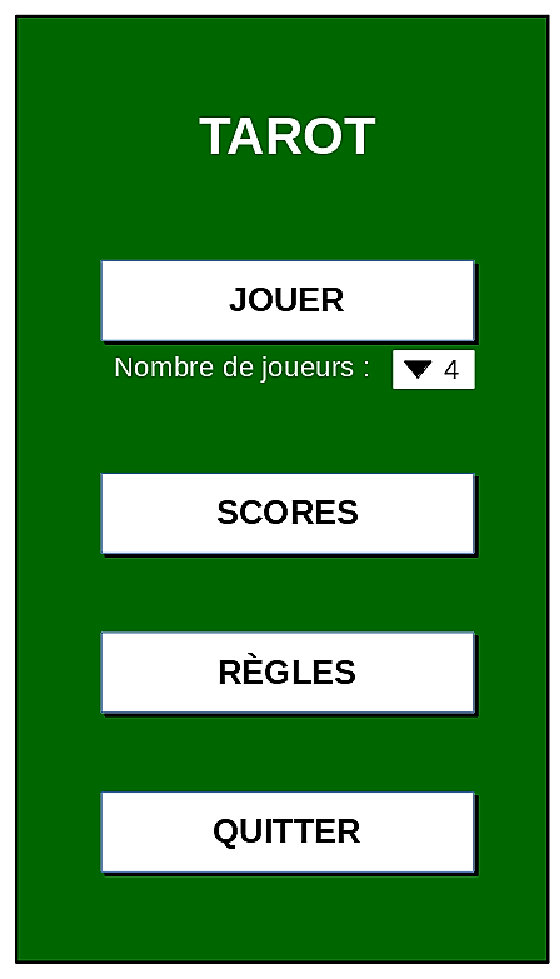
\includegraphics[scale=0.4]{maquette_ihm_1} \caption{Maquette IHM du menu principal}
\end{figure}


\begin{figure}[H]
\center 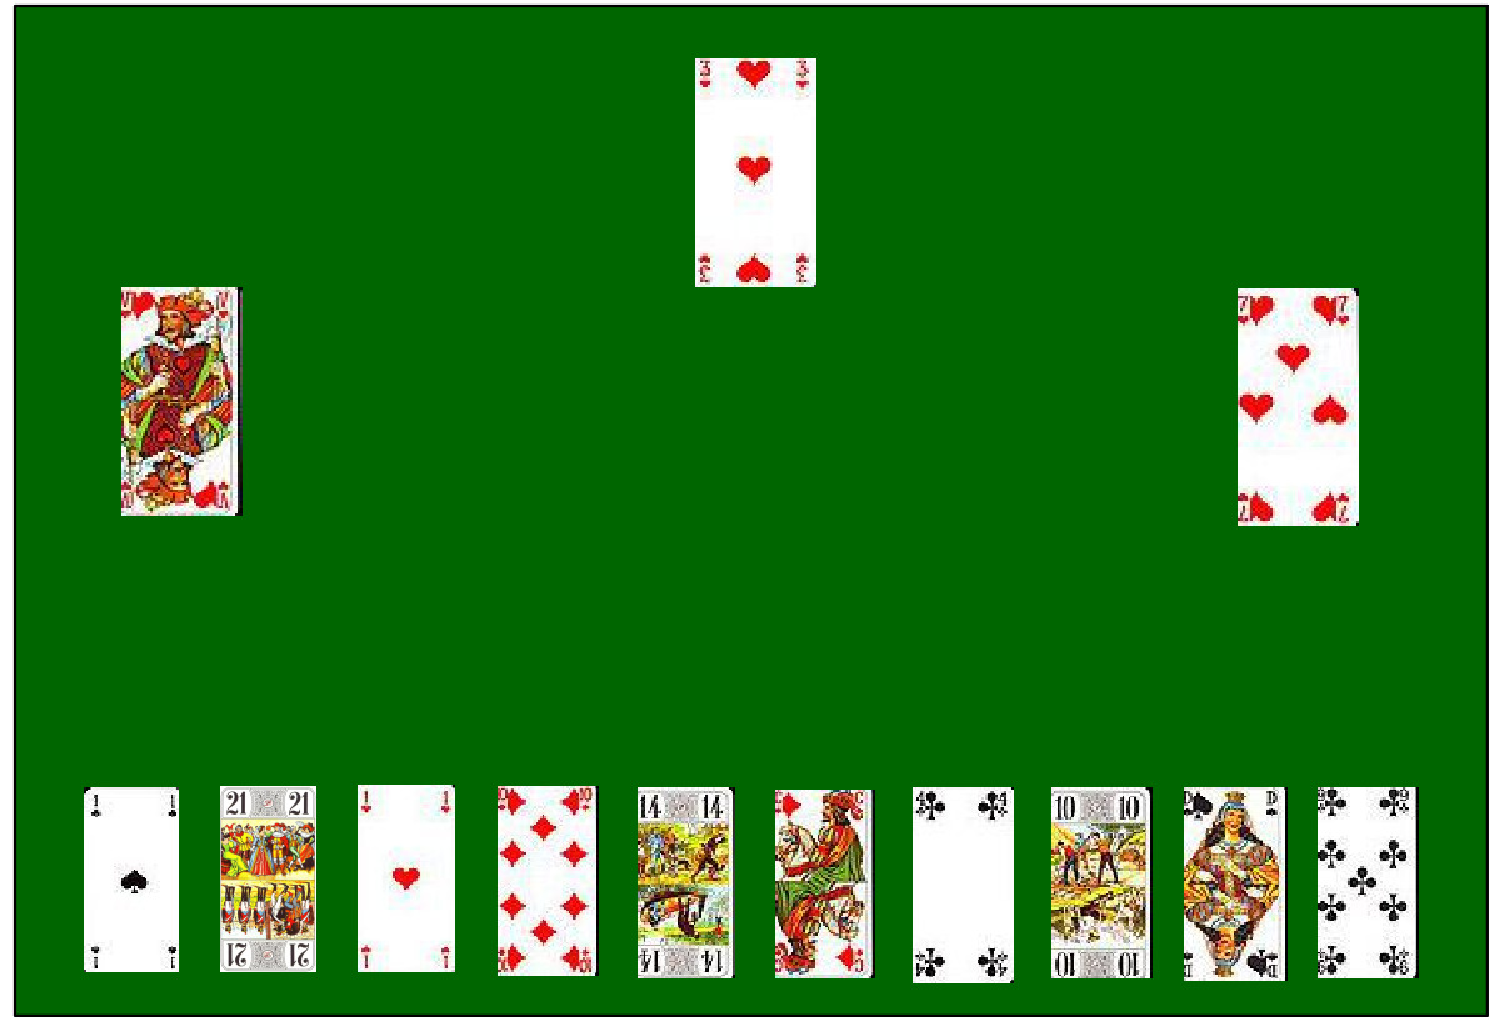
\includegraphics[scale=0.4]{maquette_ihm_2} \caption{Maquette IHM de la table de jeu}
\end{figure}


L'utilisateur choisit la carte qu'il désire jouer par un clic sur
les cartes placées en face de lui. Après chaque coup, la table de
jeu est mise à jour.


\section{Diagramme d'activité}

\begin{figure}[H]
\center 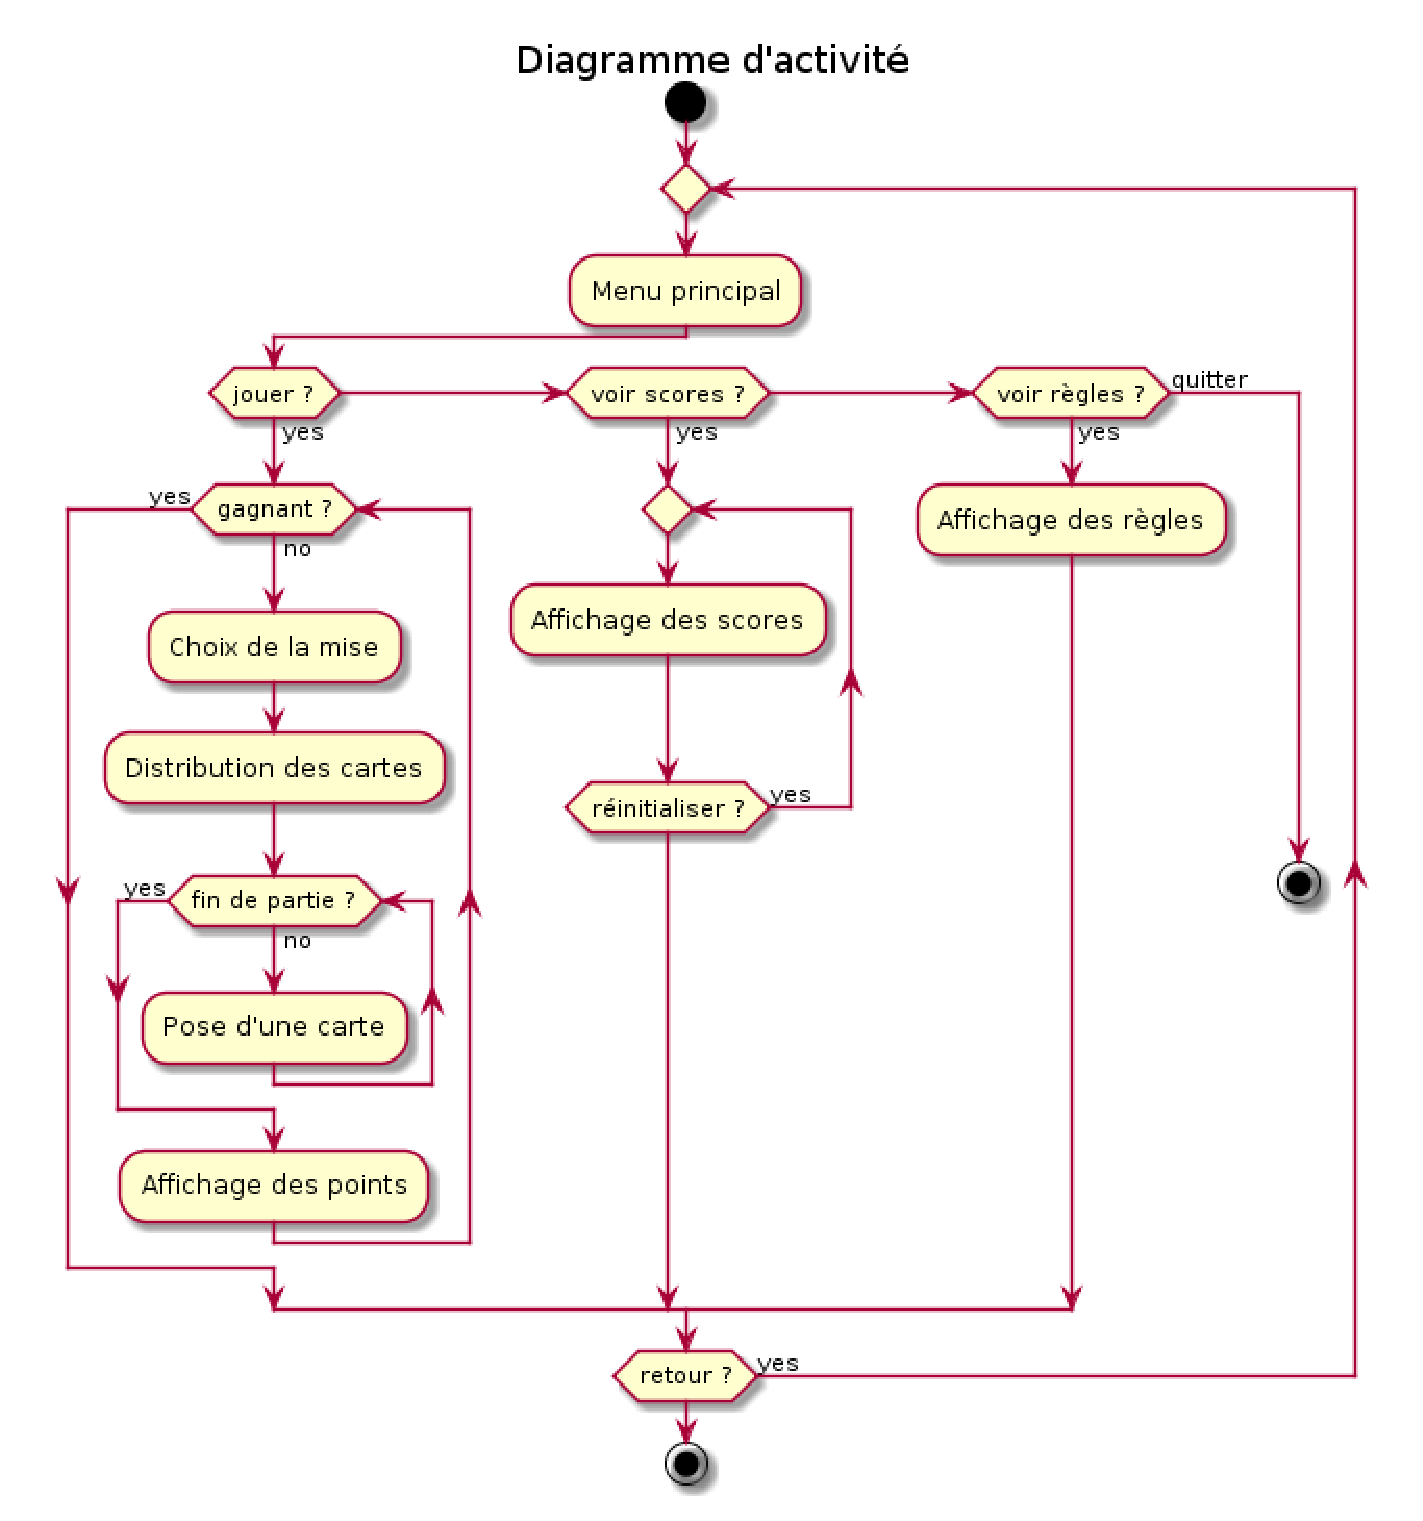
\includegraphics[scale=0.4]{diagramme_activite} \caption{Diagramme d'activité}
\end{figure}



\part{Conception}


\section{Diagramme de classe de conception}

\begin{figure}[H]
\center 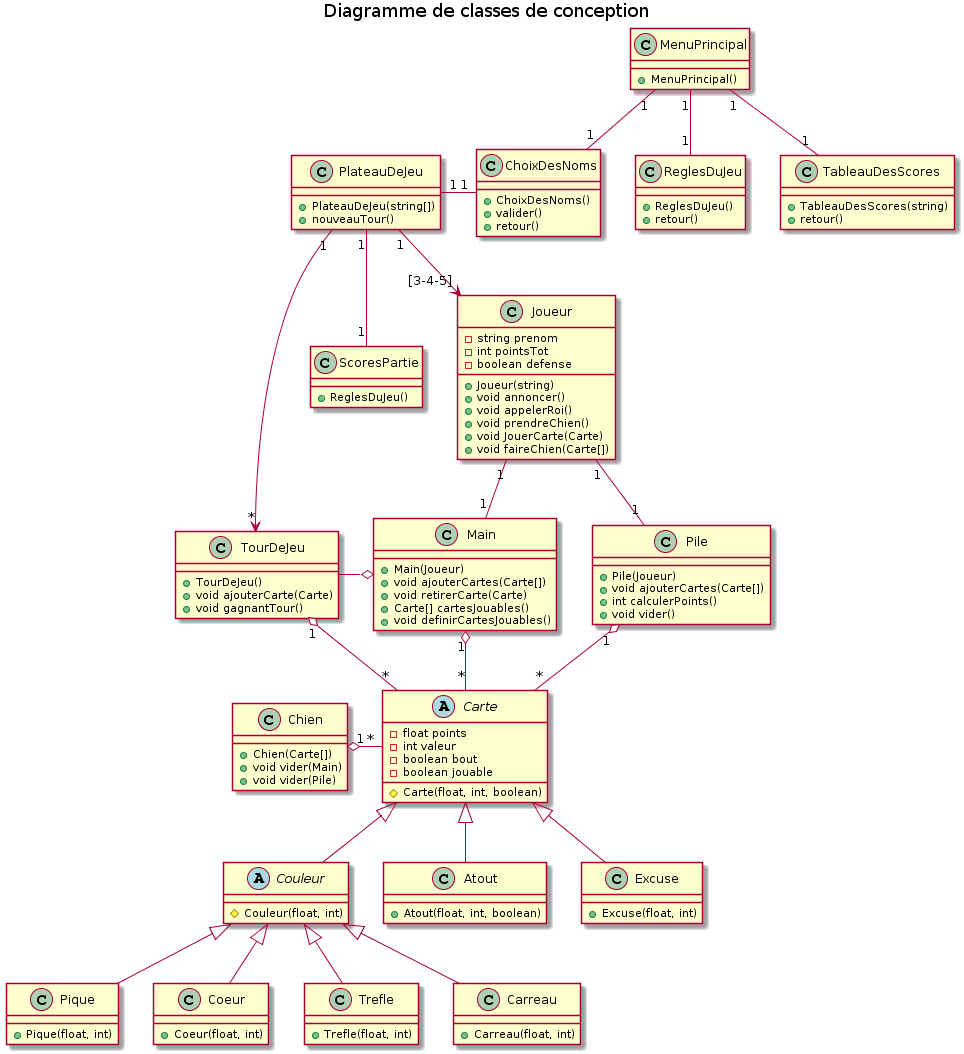
\includegraphics[scale=0.4]{diagramme_classe_conception}
\caption{Diagramme de classe de conception}
\end{figure}



\section{Diagramme de classes de participantes}

\begin{figure}[H]
\center 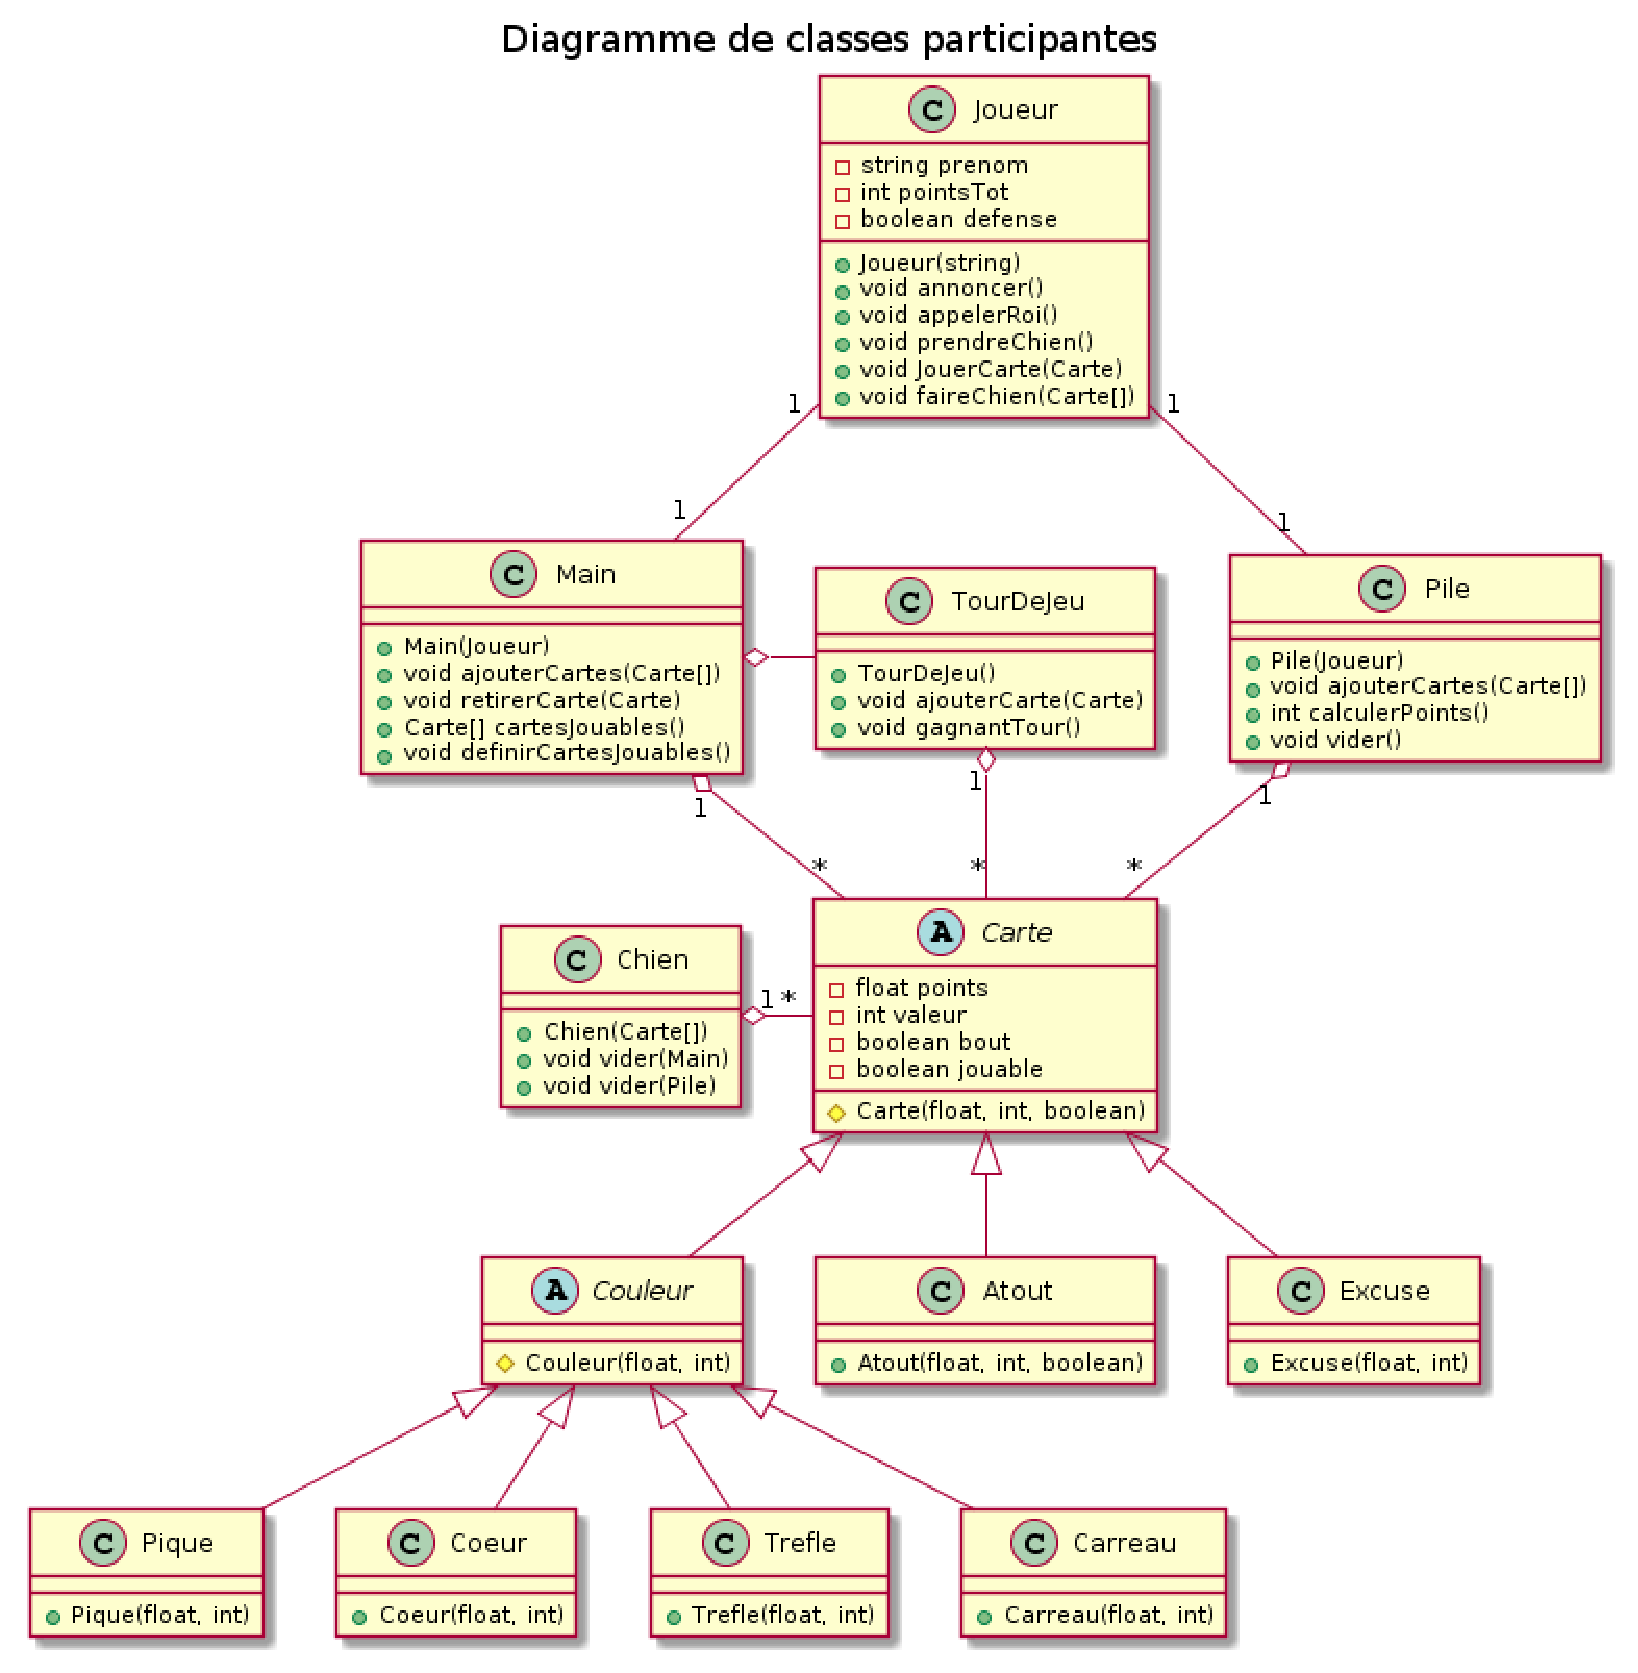
\includegraphics[scale=0.4]{diagramme_classe_particiapantes}
\caption{Diagramme de classes de participantes}
\end{figure}



\section{Diagrammes de séquence}

\begin{figure}[H]
\center 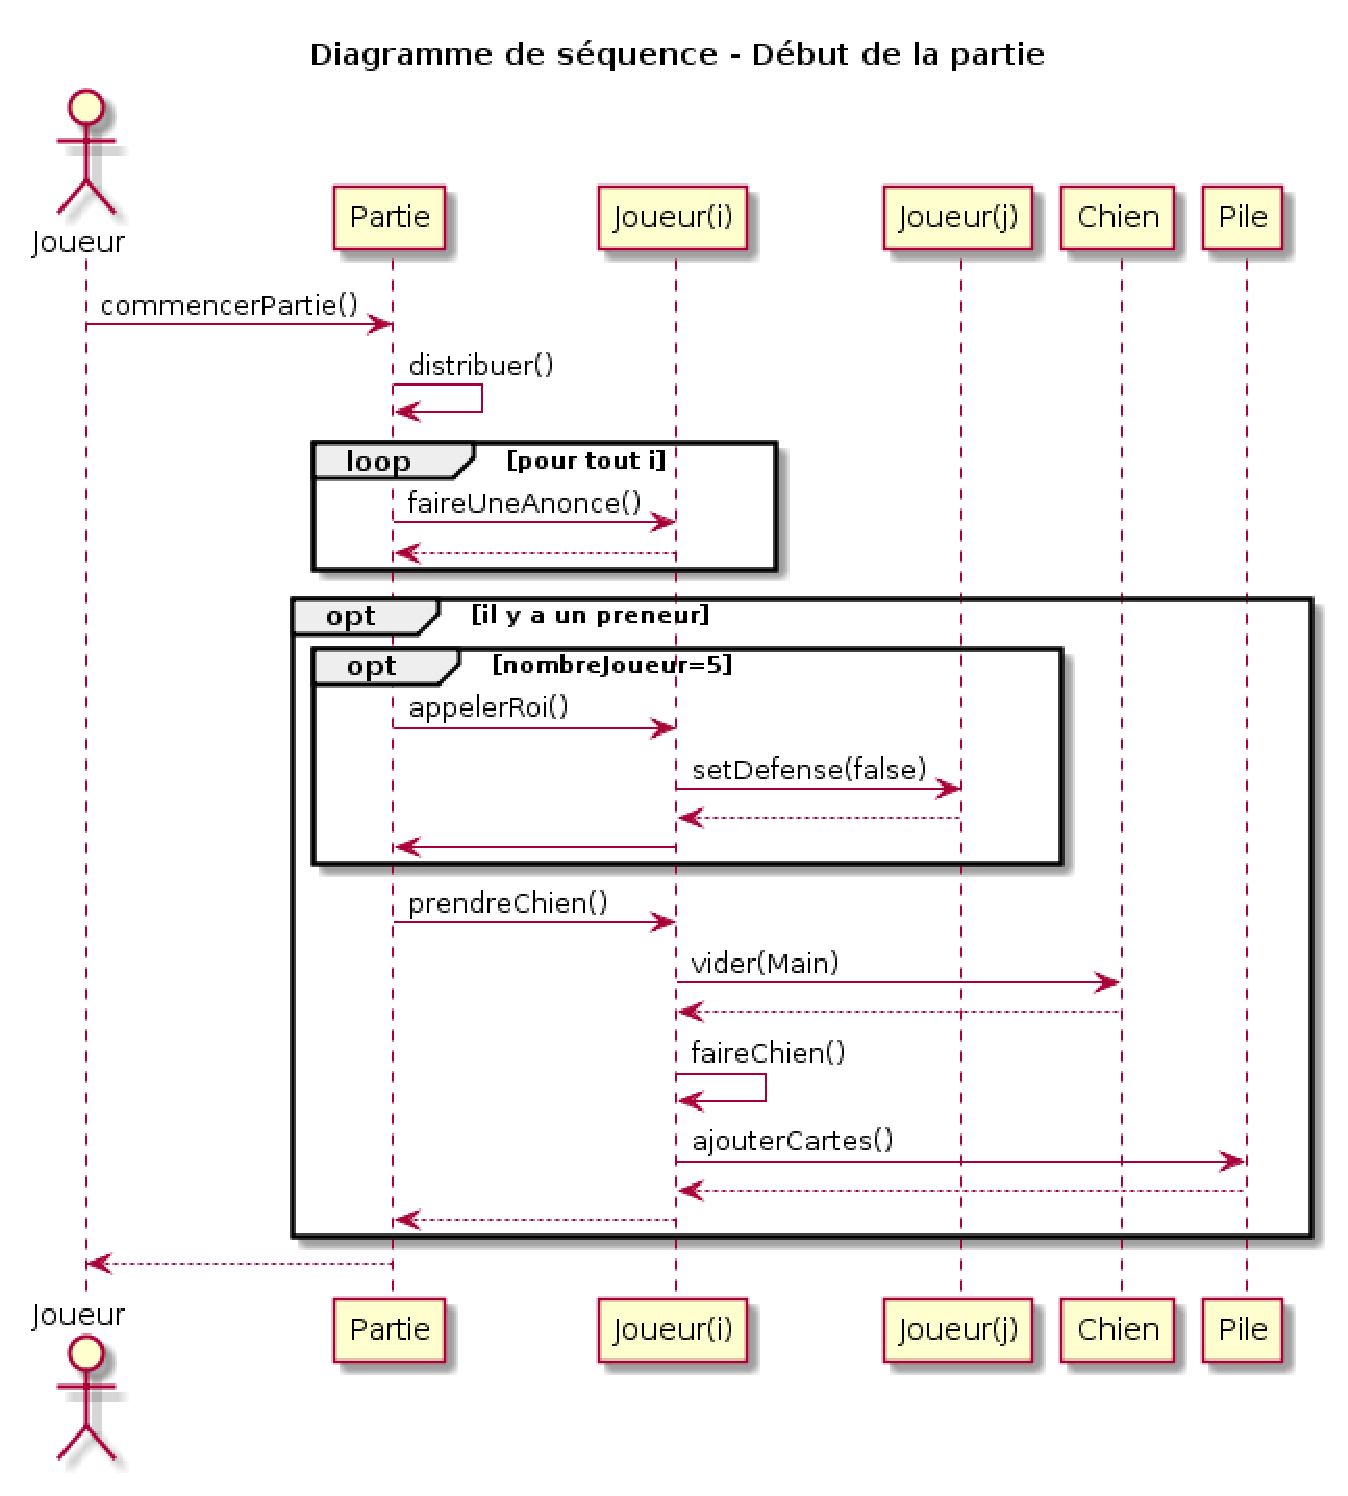
\includegraphics[scale=0.4]{diagramme_sequence_debut} \caption{Diagramme de séquence de début de partie}
\end{figure}




\begin{figure}[H]
\center 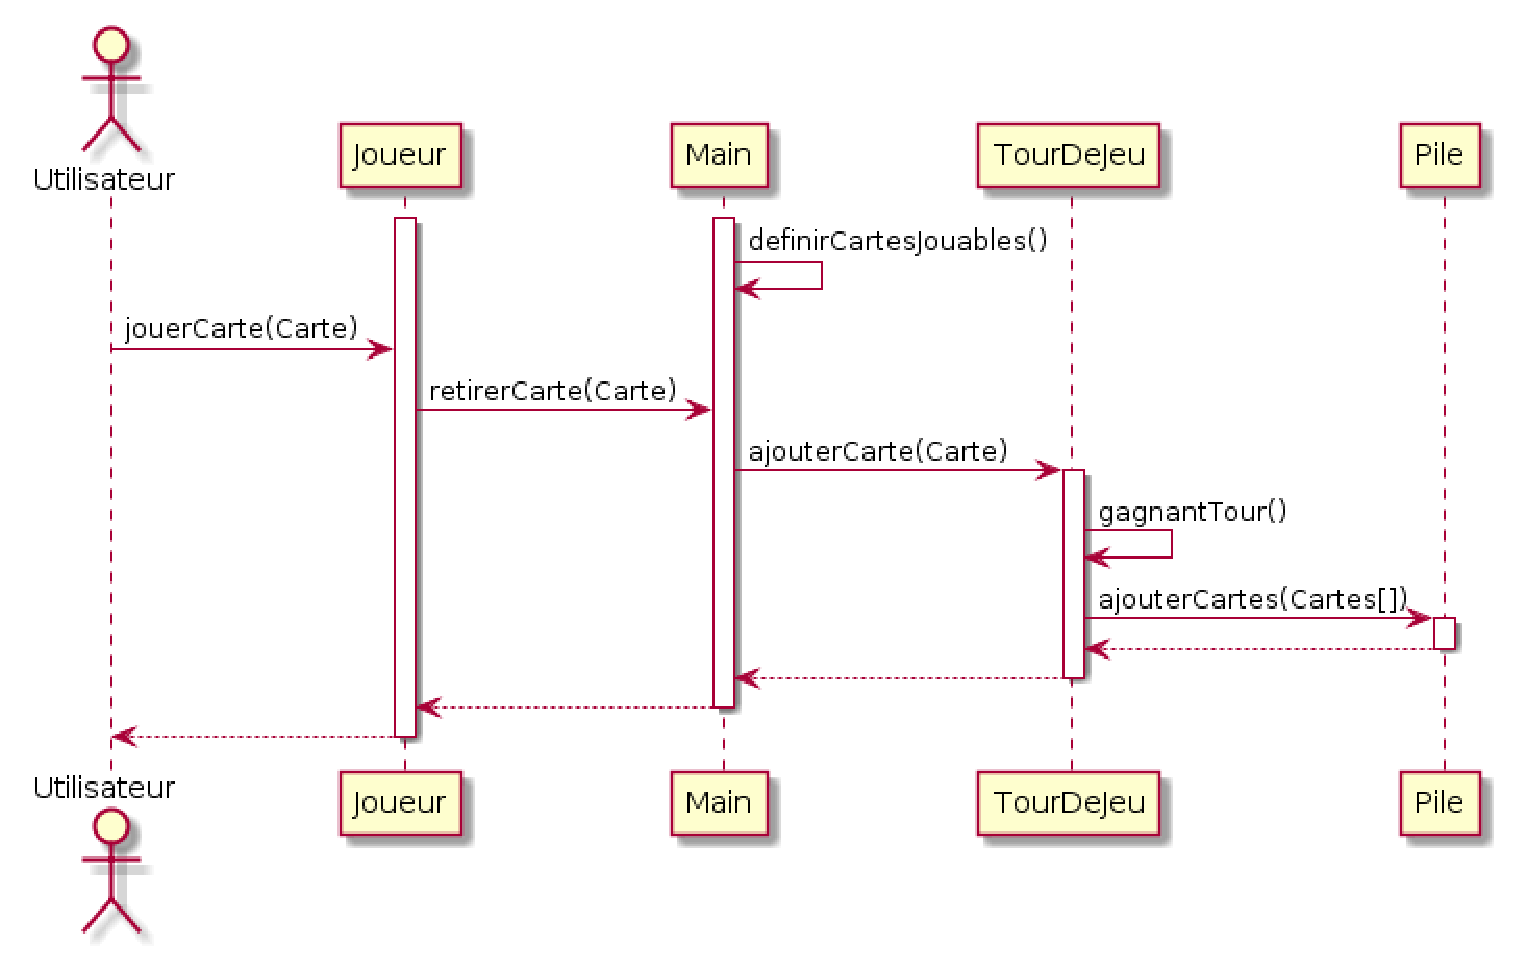
\includegraphics[scale=0.4]{diagramme_sequence_tour} \caption{Diagramme de séquence pour un tour de jeu}
\end{figure}

\end{document}
